\documentclass[runningheads]{llncs}
\usepackage[T1]{fontenc}
\usepackage{graphicx}
\usepackage{amsmath,amssymb}
\usepackage{booktabs}
\usepackage{multirow}
\usepackage{array}
\usepackage{url}
\usepackage{xcolor}
\usepackage{float}

\begin{document}

\title{PHQD: Patch-Based Hybrid Quantum Diffusion for Latent-Space Image Denoising}
\titlerunning{Patch-Based Hybrid Quantum Diffusion}

\author{B. Suhas\inst{1} \and C. Vinay Raj\inst{1} \and Guru Prasad\inst{1} \and Hosalli Prashanth\inst{1} \and Srinath Devale\inst{1}}
\authorrunning{B. Suhas et al.}

\institute{Department of Artificial Intelligence and Machine Learning,\\
Ballari Institute of Technology and Management, Ballari 583104, India\\
\texttt{3br23ai022@bitm.edu.in, 3br23ai029@bitm.edu.in, 3br23ai051@bitm.edu.in,}\\
\texttt{3br23ai057@bitm.edu.in, devalesrinath@gmail.com}}
\maketitle

\begin{abstract}
Latent-space image denoising lowers computational cost by operating on compact autoencoder features, and parameterized quantum circuits (PQCs) are increasingly explored as trainable components in such models. However, near-term quantum devices offer few qubits, and the contribution of a quantum layer is difficult to separate from that of the surrounding classical network. This work presents PHQD, a patch-based hybrid quantum--classical framework for denoising latent representations of Fashion-MNIST images. A convolutional autoencoder compresses each image into a $64\times7\times7$ latent map, which is corrupted with Gaussian noise ($\sigma=0.3$) and divided into overlapping $2\times2$ patches. A classical network converts each patch into rotation angles, a PQC processes them, and a second classical network reconstructs the denoised patch. Four 4-qubit configurations and an upgraded 6-qubit model, featuring data re-uploading, multi-basis measurement and joint training with a stitching network, are compared with multilayer perceptron (MLP), U-Net and linear regression baselines. On 10,000 test images, the 6-qubit model reduces latent mean squared error from 0.0900 to 0.0216 and achieves a peak signal-to-noise ratio (PSNR) of 25.85\,dB and a structural similarity index of 0.924, outperforming the best 4-qubit model (25.29\,dB). The classical MLP attains a higher PSNR of 25.99\,dB, while linear regression reaches 25.22\,dB, close to the 4-qubit models. Replacing the circuit output with a constant lowers the 6-qubit model to 23.63\,dB, but changes some 4-qubit models by at most 0.03\,dB. The study contributes a modular hybrid denoising pipeline and a comparative ablation analysis, showing that reliance on the quantum layer varies considerably across designs. A quantum advantage is not demonstrated, motivating parameter-matched classical controls.

\keywords{Quantum Machine Learning \and Parameterized Quantum Circuits \and Latent Image Denoising \and Hybrid Learning \and Ablation Study}
\end{abstract}
\section{Introduction}\label{sec:intro}
Image denoising, the recovery of a clean image from a corrupted observation, is a basic problem in computer vision and the core learning step of denoising diffusion models~\cite{ho}. Because operating directly on pixels is computationally expensive, latent-space methods first compress images with an autoencoder and then process the compact representation~\cite{rombach}. In parallel, variational quantum algorithms have made parameterized quantum circuits (PQCs) a common building block of hybrid quantum--classical learning~\cite{cerezo,benedetti}, raising the question of whether such circuits can serve as useful components of image reconstruction models.

The specific problem addressed in this work is the removal of Gaussian noise from the latent representation of an image using a model that contains a PQC. Noisy intermediate-scale quantum (NISQ) devices provide few qubits and are sensitive to noise~\cite{preskill}, whereas even the latent map of a $28\times28$ image in our autoencoder holds $64\times7\times7=3{,}136$ values. The representation must therefore be divided and strongly compressed before it can be encoded into a circuit. This compression, the data encoding and the measurement scheme all limit what the quantum layer can express~\cite{havlicek,schuld}, while deeper circuits can be hard to train~\cite{mcclean}.

Quantum circuits have already been used in generative and denoising models. Quantum diffusion models have been studied for image data~\cite{kolle,cacioppo} and quantum data~\cite{zhang}, and patch-based designs have enabled image generation with few qubits~\cite{huang}. Showing that a hybrid model works, however, does not reveal which of its parts is responsible for the result. Here, the classical layers contain thousands of times more trainable parameters than the circuit, and a large benchmarking study of quantum classifiers found that conclusions depend strongly on the baselines and that removing quantum properties does not necessarily reduce performance~\cite{bowles}. For patch-based latent denoising, the effects of circuit depth, encoding and readout, and the dependence of the model on its quantum layer, have not been examined closely. This matters because quantum resources are scarce and costly to simulate or access: without strong baselines and ablation tests, an improvement caused by a wider classical network or an extra refinement stage may wrongly be credited to the circuit.

We therefore present PHQD, a patch-based hybrid quantum--classical framework for latent image denoising on Fashion-MNIST~\cite{fmnist}. A convolutional autoencoder produces the latent map, which is corrupted with Gaussian noise and divided into overlapping patches. A classical network converts each patch into rotation angles, a PQC processes them, and the output is mapped back to patch space; the patches are then recombined and decoded. The objectives of this study are:
\begin{enumerate}
\item To design a modular hybrid pipeline for patch-wise denoising of latent image representations.
\item To compare the effects of circuit depth, data encoding and measurement strategy across several quantum configurations.
\item To determine, using classical baselines and ablation tests, how strongly performance depends on the quantum layer.
\end{enumerate}

The main contributions of this paper are:
\begin{itemize}
\item An end-to-end implementation combining a convolutional autoencoder, overlapping patch processing, a batched PQC denoiser and a stitching network.
\item A comparison of four 4-qubit configurations with a 6-qubit model that uses data re-uploading, three-basis measurement and joint refinement.
\item An evaluation on held-out Fashion-MNIST test images against multilayer perceptron, U-Net and linear regression baselines.
\item An ablation analysis showing that reliance on the circuit output differs considerably between configurations, together with a stitching-network control indicating that part of the 6-qubit model's advantage may arise from classical refinement.
\end{itemize}


\section{Related Work}\label{sec:related}
Diffusion models learn to reverse a gradual noising process and give high-quality image synthesis~\cite{ho}. Latent diffusion makes them cheaper by denoising the compact latent space of an autoencoder instead of pixels~\cite{rombach}. Both are fully classical, and we adopt only the idea of denoising a latent representation, with a U-Net~\cite{unet} as a convolutional baseline.

Several studies place quantum circuits inside diffusion models. K\"olle et al.~\cite{kolle} showed that a dense circuit with about 1,000 parameters beats equal-size classical networks on $8\times8$ MNIST, although a much larger U-Net is still best. Cacioppo et al.~\cite{cacioppo} used circuits as the denoiser and found that working on autoencoder latents gives far better FID than a fully quantum model, but only on small MNIST images and with a mostly qualitative classical comparison. Zhang et al.~\cite{zhang} and Parigi et al.~\cite{parigi} studied quantum states and toy data, and Huang et al.~\cite{huang} generated digit images with a quantum GAN on hardware. These works show that quantum circuits can be trained for generation and denoising, but they use small data, quantum data or a different task. None of them is a patch-based latent image denoiser.

Other studies deal with circuit design. Feature-map encodings~\cite{havlicek} and data re-uploading~\cite{salinas,schuld} increase what a circuit can represent, and we use both ideas. Deep random circuits can have vanishing gradients~\cite{mcclean}, so we keep our circuits shallow. Bowles et al.~\cite{bowles} found that simple classical models often beat quantum ones and that removing entanglement often does not hurt, which is why we add strong classical baselines and remove the circuit output in an ablation.

In short, earlier work shows that quantum denoisers are possible, but it does not tell which part of a hybrid model gives the gain. PHQD fills this gap by comparing several circuit designs with classical baselines on patch-wise latent denoising and by measuring the effect of removing the circuit. Table~\ref{tab:related} summarises the closest studies.

\begin{table}[t]
\caption{Summary of closely related studies.}\label{tab:related}
\centering\scriptsize
\renewcommand{\arraystretch}{1.2}
\begin{tabular}{@{}>{\raggedright\arraybackslash}p{0.22\textwidth}>{\raggedright\arraybackslash}p{0.25\textwidth}>{\raggedright\arraybackslash}p{0.45\textwidth}@{}}
\toprule
Study & Method & Limitation for our problem\\
\midrule
Rombach et al.~\cite{rombach} & Classical latent diffusion & No quantum component\\
K\"olle et al.~\cite{kolle} & Circuits in diffusion & Small MNIST; larger U-Net still best\\
Cacioppo et al.~\cite{cacioppo} & Circuit denoiser, latent variant & Small scale; limited classical comparison\\
Zhang et al.~\cite{zhang} & Step-wise quantum diffusion & Quantum data; few qubits\\
Huang et al.~\cite{huang} & Quantum GAN on hardware & Simple benchmark; not a denoiser\\
Bowles et al.~\cite{bowles} & Large benchmarking study & Classification only\\
\bottomrule
\end{tabular}
\end{table}
\section{Preliminaries}\label{sec:prelim}
This section gives the basic ideas behind PHQD.

A convolutional autoencoder compresses an image into a small latent map and rebuilds it from that map~\cite{rombach}. Ours maps a $28\times28$ image to a latent map $z$ of size $64\times7\times7$. We add Gaussian noise, $\tilde z=z+\sigma\epsilon$ with $\sigma=0.3$, as in diffusion models~\cite{ho}, and train a denoiser to recover $z$ by minimising the mean squared error (MSE). Because the latent map has 3,136 values, it is split into $2\times2$ patches with stride one, which gives 36 overlapping patches of 256 values. Each patch is denoised separately, and overlapping values are averaged when the map is put back together.

A qubit is a two-level quantum system, and quantum gates change its state. A rotation gate $R_Y(\theta)$ turns a number $\theta$ into a state change, and a CNOT gate links two qubits through entanglement. Measuring a qubit gives an expectation value between $-1$ and $1$. A parameterized quantum circuit (PQC) encodes input data as gate angles, applies layers of trainable gates and returns such expectation values~\cite{cerezo,benedetti}. Its weights are trained by gradient descent like network weights. We simulate all circuits on a classical computer, so hardware noise~\cite{preskill} is not included, and we keep the circuits shallow because deep ones can be hard to train~\cite{mcclean}.

We compare three ways to feed data into a circuit. Angle encoding sets one rotation angle per feature. The IQP-style encoding~\cite{havlicek} adds two-qubit interactions between features. Data re-uploading~\cite{salinas} repeats the encoding in every layer, which lets the model represent more complex functions~\cite{schuld}. We can also measure $X$, $Y$ and $Z$ on each qubit instead of $Z$ only, which triples the number of outputs.

In our hybrid denoiser, a classical network turns each patch into $n$ angles, the PQC processes them, and a second classical network, with a linear shortcut from the input, rebuilds the patch. A small stitching network can then refine the rebuilt latent map. As baselines we use a multilayer perceptron (MLP) on patches and a U-Net~\cite{unet} on the full latent map, which show how far a purely classical model can go.

We measure quality with MSE, the peak signal-to-noise ratio (PSNR) and the structural similarity index (SSIM), and with the Fr\'echet Inception Distance (FID), which compares the feature statistics of real and reconstructed images. Lower MSE and FID and higher PSNR and SSIM are better.

\section{Proposed PHQD Framework}\label{sec:method}

\subsection{Overview}
PHQD removes Gaussian noise from the latent representation of an image, one small patch at a time, so that each patch fits a few-qubit circuit. Figure~\ref{fig:architecture} shows the workflow. A convolutional autoencoder compresses a Fashion-MNIST image into a latent map, Gaussian noise is added, and the noisy map is cut into overlapping patches. A hybrid quantum--classical model denoises each patch, the patches are averaged back into a latent map, an optional stitching network refines it, and the decoder produces the image.

\begin{figure*}[t]
\centering
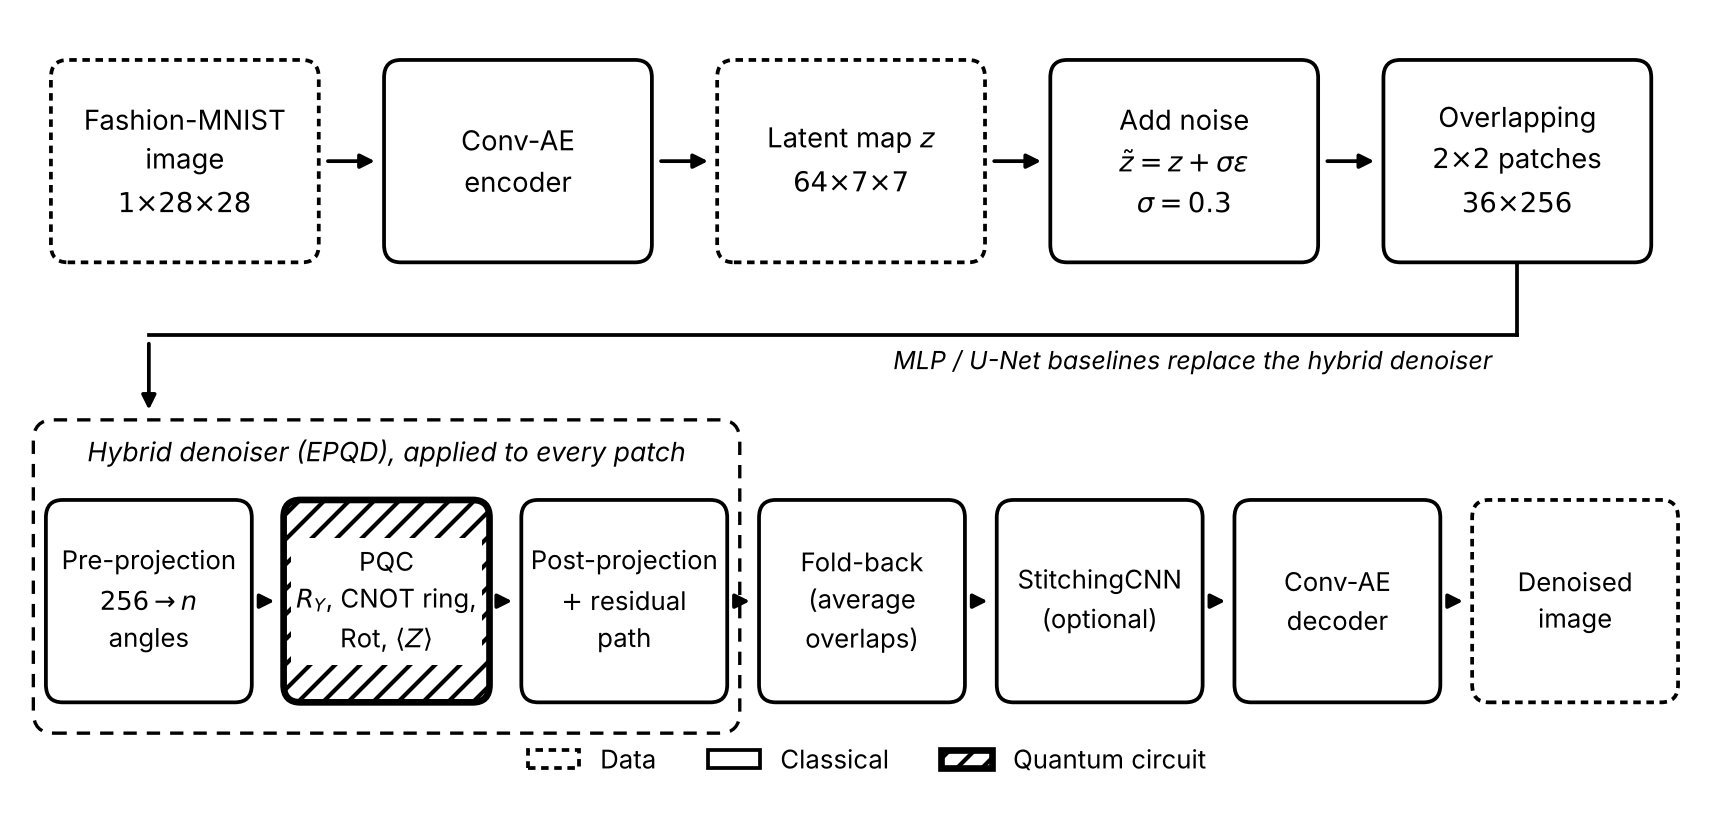
\includegraphics[width=0.92\textwidth]{phqd_architecture_bw.png}
\caption{Overall pipeline of the proposed PHQD framework.}
\label{fig:architecture}
\end{figure*}

\subsection{Data and Preprocessing}
We use Fashion-MNIST~\cite{fmnist} with 60{,}000 training and 10{,}000 test grayscale images of $28\times28$ pixels. Pixels are normalized with mean 0.5 and standard deviation 0.5, so they lie in $[-1,1]$. The encoder of the trained, frozen autoencoder maps each image to a latent map $z\in\mathbb{R}^{64\times7\times7}$, which is corrupted as
\begin{equation}
    \tilde z = z+\sigma\epsilon,\qquad \epsilon\sim\mathcal{N}(0,I),\quad \sigma=0.3.
\end{equation}
A $2\times2$ window with stride one over the $7\times7$ grid gives 36 overlapping patches per image, each flattened to $64\times2\times2=256$ values.

\subsection{Convolutional Autoencoder}
The encoder has two strided convolutions ($1\rightarrow32\rightarrow64$ channels, $4\times4$ kernel, stride 2, padding 1), each followed by batch normalization and LeakyReLU, and maps an image to a $64\times7\times7$ latent map. The decoder mirrors it with two transposed convolutions and a Tanh output. It is trained with MSE loss and Adam (learning rate $10^{-3}$, cosine annealing) for 20 epochs with batch size 128.

\subsection{EPQD Denoiser}
For each patch $p$, a classical pre-projection ($256\rightarrow128\rightarrow n$) with a Tanh output gives $n$ values that are mapped to rotation angles in $[0,\pi]$:
\begin{equation}
    a(p)=\frac{\pi}{2}\left(g_{\mathrm{pre}}(p)+1\right).
\end{equation}
The circuit applies $R_Y(a_i)$ on each of $n$ qubits. Each of $L$ variational layers then applies a ring of CNOT gates followed by a trainable \texttt{Rot} gate on every qubit, and the circuit returns the Pauli-$Z$ expectations
\begin{equation}
    q(p)=\left(\langle Z_0\rangle,\ldots,\langle Z_{n-1}\rangle\right).
\end{equation}
A classical post-projection ($n\rightarrow128\rightarrow256\rightarrow256$) and a learned linear residual path from the input give the denoised patch:
\begin{equation}
    \hat p=g_{\mathrm{post}}(q(p))+W_rp+b_r.
\end{equation}
The circuit is simulated with PennyLane on \texttt{default.qubit} using backpropagation. The IQP variant (EPQD-IQP) replaces the first step with Hadamard gates, data-dependent $R_Z$ rotations and Ising-$ZZ$ interactions. Table~\ref{tab:configs} lists the four 4-qubit configurations.

\begin{table}[t]
\centering
\caption{Standard EPQD quantum configurations.}
\label{tab:configs}
\begin{tabular}{lccc}
\toprule
\textbf{Model} & \textbf{Qubits} & \textbf{Layers} & \textbf{Ansatz}\\
\midrule
EPQD-S & 4 & 1 & Basic ring + Rot\\
EPQD-M & 4 & 2 & Basic ring + Rot\\
EPQD-L & 4 & 3 & Basic ring + Rot\\
EPQD-IQP & 4 & 2 & IQP-style + ring + Rot\\
\bottomrule
\end{tabular}
\end{table}

\subsection{EPQD-6Q-V2}
EPQD-6Q-V2 uses six qubits and three layers, re-uploads the input in every layer, and reads out $X$, $Y$ and $Z$ on each qubit, which gives 18 features for the post-projection:
\begin{equation}
    q_{\mathrm{XYZ}}\in\mathbb{R}^{18}.
\end{equation}
It is trained jointly with the stitching network using the loss
\begin{equation}
    \mathcal{L}_{\mathrm{V2}}=
    \mathcal{L}_{\mathrm{latent\text{-}MSE}}
    +0.5\,\mathcal{L}_{\mathrm{image\text{-}MSE}}
    +0.2\left(1-\operatorname{SSIM}(\hat x,x)\right).
\end{equation}

\subsection{Stitching Network and Fold-Back}
Denoised patches are placed back at their grid positions, and overlapping estimates are averaged:
\begin{equation}
    \hat z(c,h,w)=
    \frac{1}{|\mathcal{I}(h,w)|}\sum_{p\in\mathcal{I}(h,w)}\hat p(c,h-h_p,w-w_p),
\end{equation}
where $\mathcal{I}(h,w)$ is the set of patches covering position $(h,w)$. The optional StitchingCNN is a classical network (a $1\times1$ stem, three residual blocks with two $3\times3$ convolutions each, and a $1\times1$ Tanh head with a skip connection) that refines this map. It is first trained alone to remove noise with standard deviation 0.15 from latent maps, for 15 epochs with Adam at $10^{-3}$. The decoder then turns the latent map into the denoised image.

\subsection{Training}
The standard EPQD models are trained in two stages with MSE loss, Adam, cosine annealing and batch size 128. In the warm-up, the quantum weights are frozen and a linear bypass replaces the circuit, so that the classical layers train for 10 epochs at learning rate $10^{-3}$. The bypass is then removed and the whole model is fine-tuned for 8 epochs at $3\times10^{-3}$ on at most 8{,}000 patches. EPQD-6Q-V2 uses three phases of 15, 8 and 6 epochs with learning rates $10^{-3}$, $2\times10^{-3}$ and $5\times10^{-4}$, the last one jointly with the stitching network.

\subsection{Baselines and Evaluation}
The MLP baseline denoises flattened 256-value patches ($256\rightarrow512\rightarrow512\rightarrow256\rightarrow256$ with LayerNorm, GELU, dropout 0.1 and a residual connection). The U-Net baseline denoises the full $64\times7\times7$ latent map with two encoder blocks (64 and 128 channels), a 256-channel bottleneck and a decoder with skip connections. Both are trained for 20 epochs with MSE loss, Adam at $10^{-3}$ and batch size 128. All denoisers receive the same noisy latent maps with $\sigma=0.3$, and the decoded clean and noisy latent maps serve as upper and lower references.

We report MSE, PSNR $=10\log_{10}(1/\mathrm{MSE})$ and SSIM between the decoded and original images mapped to $[0,1]$ on test images, and the Fr\'echet Inception Distance (FID) from Inception-V3 features of 1{,}000 test images. Lower MSE and FID and higher PSNR and SSIM are better.

\section{Experimental Setup}\label{sec:setup}

\subsection{Data and Noise}
All experiments use Fashion-MNIST~\cite{fmnist}, with 60{,}000 training and 10{,}000 test grayscale $28\times28$ images, loaded through \texttt{torchvision}. Pixels are normalized with mean 0.5 and standard deviation 0.5. No validation split is held out, and the test split is used for monitoring and final evaluation. The autoencoder is trained on the full training split. To keep the circuit simulation tractable, the denoisers use only part of the data: the EPQD models use 30 training batches and 8 test batches of latent patches, with at most 8{,}000 patches for quantum fine-tuning, and the MLP and U-Net use 50 training and 10 test batches. Noise is added to latent features, not to pixels, with $\tilde p=p+\epsilon$ and $\epsilon\sim\mathcal{N}(0,0.3^2I)$. Only the standalone stitching network is trained with a smaller noise level of 0.15.

\subsection{Environment and Configuration}
The models are written in PyTorch (2.1 or later), and the circuits in PennyLane (0.40 or later) run on the classical \texttt{default.qubit} simulator, so no quantum hardware or hardware noise is involved. Training uses a GPU when available and otherwise the CPU, and the FID evaluation runs on the CPU. The experiments were run on [hardware description]. All models use Adam with cosine annealing, and Table~\ref{tab:hyper} lists their epochs, learning rates and batch sizes. Each model is trained once with no repetitions, and a fixed seed of 42 is used for the FID evaluation and the V2 benchmark noise. The small differences between the 4-qubit models should therefore not be read as statistically established.

\begin{table}[t]
\centering
\caption{Training settings. Multi-stage models list one value per stage.}
\label{tab:hyper}
\begin{tabular}{lccc}
\toprule
\textbf{Model} & \textbf{Epochs} & \textbf{Learning rate} & \textbf{Batch}\\
\midrule
Conv-AE & 20 & $10^{-3}$ & 128\\
StitchingCNN & 15 & $10^{-3}$ & 128\\
MLP, U-Net & 20 & $10^{-3}$ & 128\\
EPQD (warm-up, fine-tune) & 10, 8 & $10^{-3}$, $3\times10^{-3}$ & 128\\
EPQD-6Q-V2 (3 phases) & 15, 8, 6 & $10^{-3}$, $2\times10^{-3}$, $5\times10^{-4}$ & 128, 128, 16\\
\bottomrule
\end{tabular}
\end{table}

\subsection{Baselines and Metrics}
The four 4-qubit EPQD models and EPQD-6Q-V2 are compared with the patch-wise MLP and the U-Net. All of them receive the same noisy latent maps from the same frozen autoencoder and use MSE as the training loss. The decoded clean latent map is the best possible result, and the decoded noisy latent map is the lower reference.

Images are decoded and mapped to $[0,1]$ before evaluation. We report the mean squared error, $\mathrm{MSE}=\frac{1}{N}\sum_i(x_i-\hat x_i)^2$, and the peak signal-to-noise ratio, $\mathrm{PSNR}=10\log_{10}(1/\mathrm{MSE})$. We also report the structural similarity index (SSIM), which compares local luminance, contrast and structure. The Fr\'echet Inception Distance (FID) compares the Inception-V3 feature distributions of real and reconstructed images,
\begin{equation}
    \operatorname{FID}=\|\mu_r-\mu_g\|_2^2+
    \operatorname{Tr}\!\left(\Sigma_r+\Sigma_g-2(\Sigma_r\Sigma_g)^{1/2}\right),
\end{equation}
and is computed on 1{,}000 test images. The V2 benchmark uses 64 test images and also reports RMSE, mean absolute error and cosine similarity. Lower MSE and FID and higher PSNR and SSIM indicate better results.

\section{Results and Discussion}\label{sec:results}

\subsection{Quantitative Results}
Table~\ref{tab:results} compares all models on 32 test images after decoding, with latent noise $\sigma=0.3$. The noisy input reaches an MSE of 0.00416, and the clean autoencoder output (0.00026) is the best any latent denoiser can reach. All denoisers improve on the noisy input. The MLP is the best denoiser on MSE, PSNR and SSIM. The four EPQD models are second and are close to each other, and EPQD-L is the best of them. The U-Net has the highest MSE of the denoisers, but it has the best FID, followed by the MLP. The EPQD models reduce the FID from 89.7 to about 70, which is worse than both classical baselines.

\begin{table}[t]
\centering
\caption{Image-level results on 32 test images (MSE, PSNR, SSIM) and FID on 1{,}000 test images. Best denoiser in bold.}
\label{tab:results}
\begin{tabular}{lcccc}
\toprule
\textbf{Model} & \textbf{MSE} & \textbf{PSNR (dB)} & \textbf{SSIM} & \textbf{FID}\\
\midrule
Conv-AE (clean) & 0.00026 & 35.85 & 0.989 & 9.0\\
Noisy latent & 0.00416 & 23.80 & 0.897 & 89.7\\
\midrule
MLP & \textbf{0.00245} & \textbf{26.12} & \textbf{0.931} & 58.4\\
U-Net & 0.00373 & 24.28 & 0.918 & \textbf{51.2}\\
EPQD-S (4q, 1 layer) & 0.00300 & 25.23 & 0.919 & 70.0\\
EPQD-M (4q, 2 layers) & 0.00298 & 25.26 & 0.920 & 70.0\\
EPQD-L (4q, 3 layers) & 0.00294 & 25.32 & 0.920 & 69.7\\
EPQD-IQP (4q, 2 layers) & 0.00301 & 25.22 & 0.919 & 70.1\\
EPQD-6Q-V2 & -- & -- & -- & --\\
\bottomrule
\end{tabular}
\end{table}


At patch level, the noisy input has an MSE of 0.0915. The EPQD models reduce it to 0.0313 (S), 0.0312 (M), 0.0308 (L) and 0.0314 (IQP), whereas the MLP reaches 0.0257. Patch-level and image-level values are measured in different spaces and should not be compared directly.


\begin{figure*}[t]
\centering
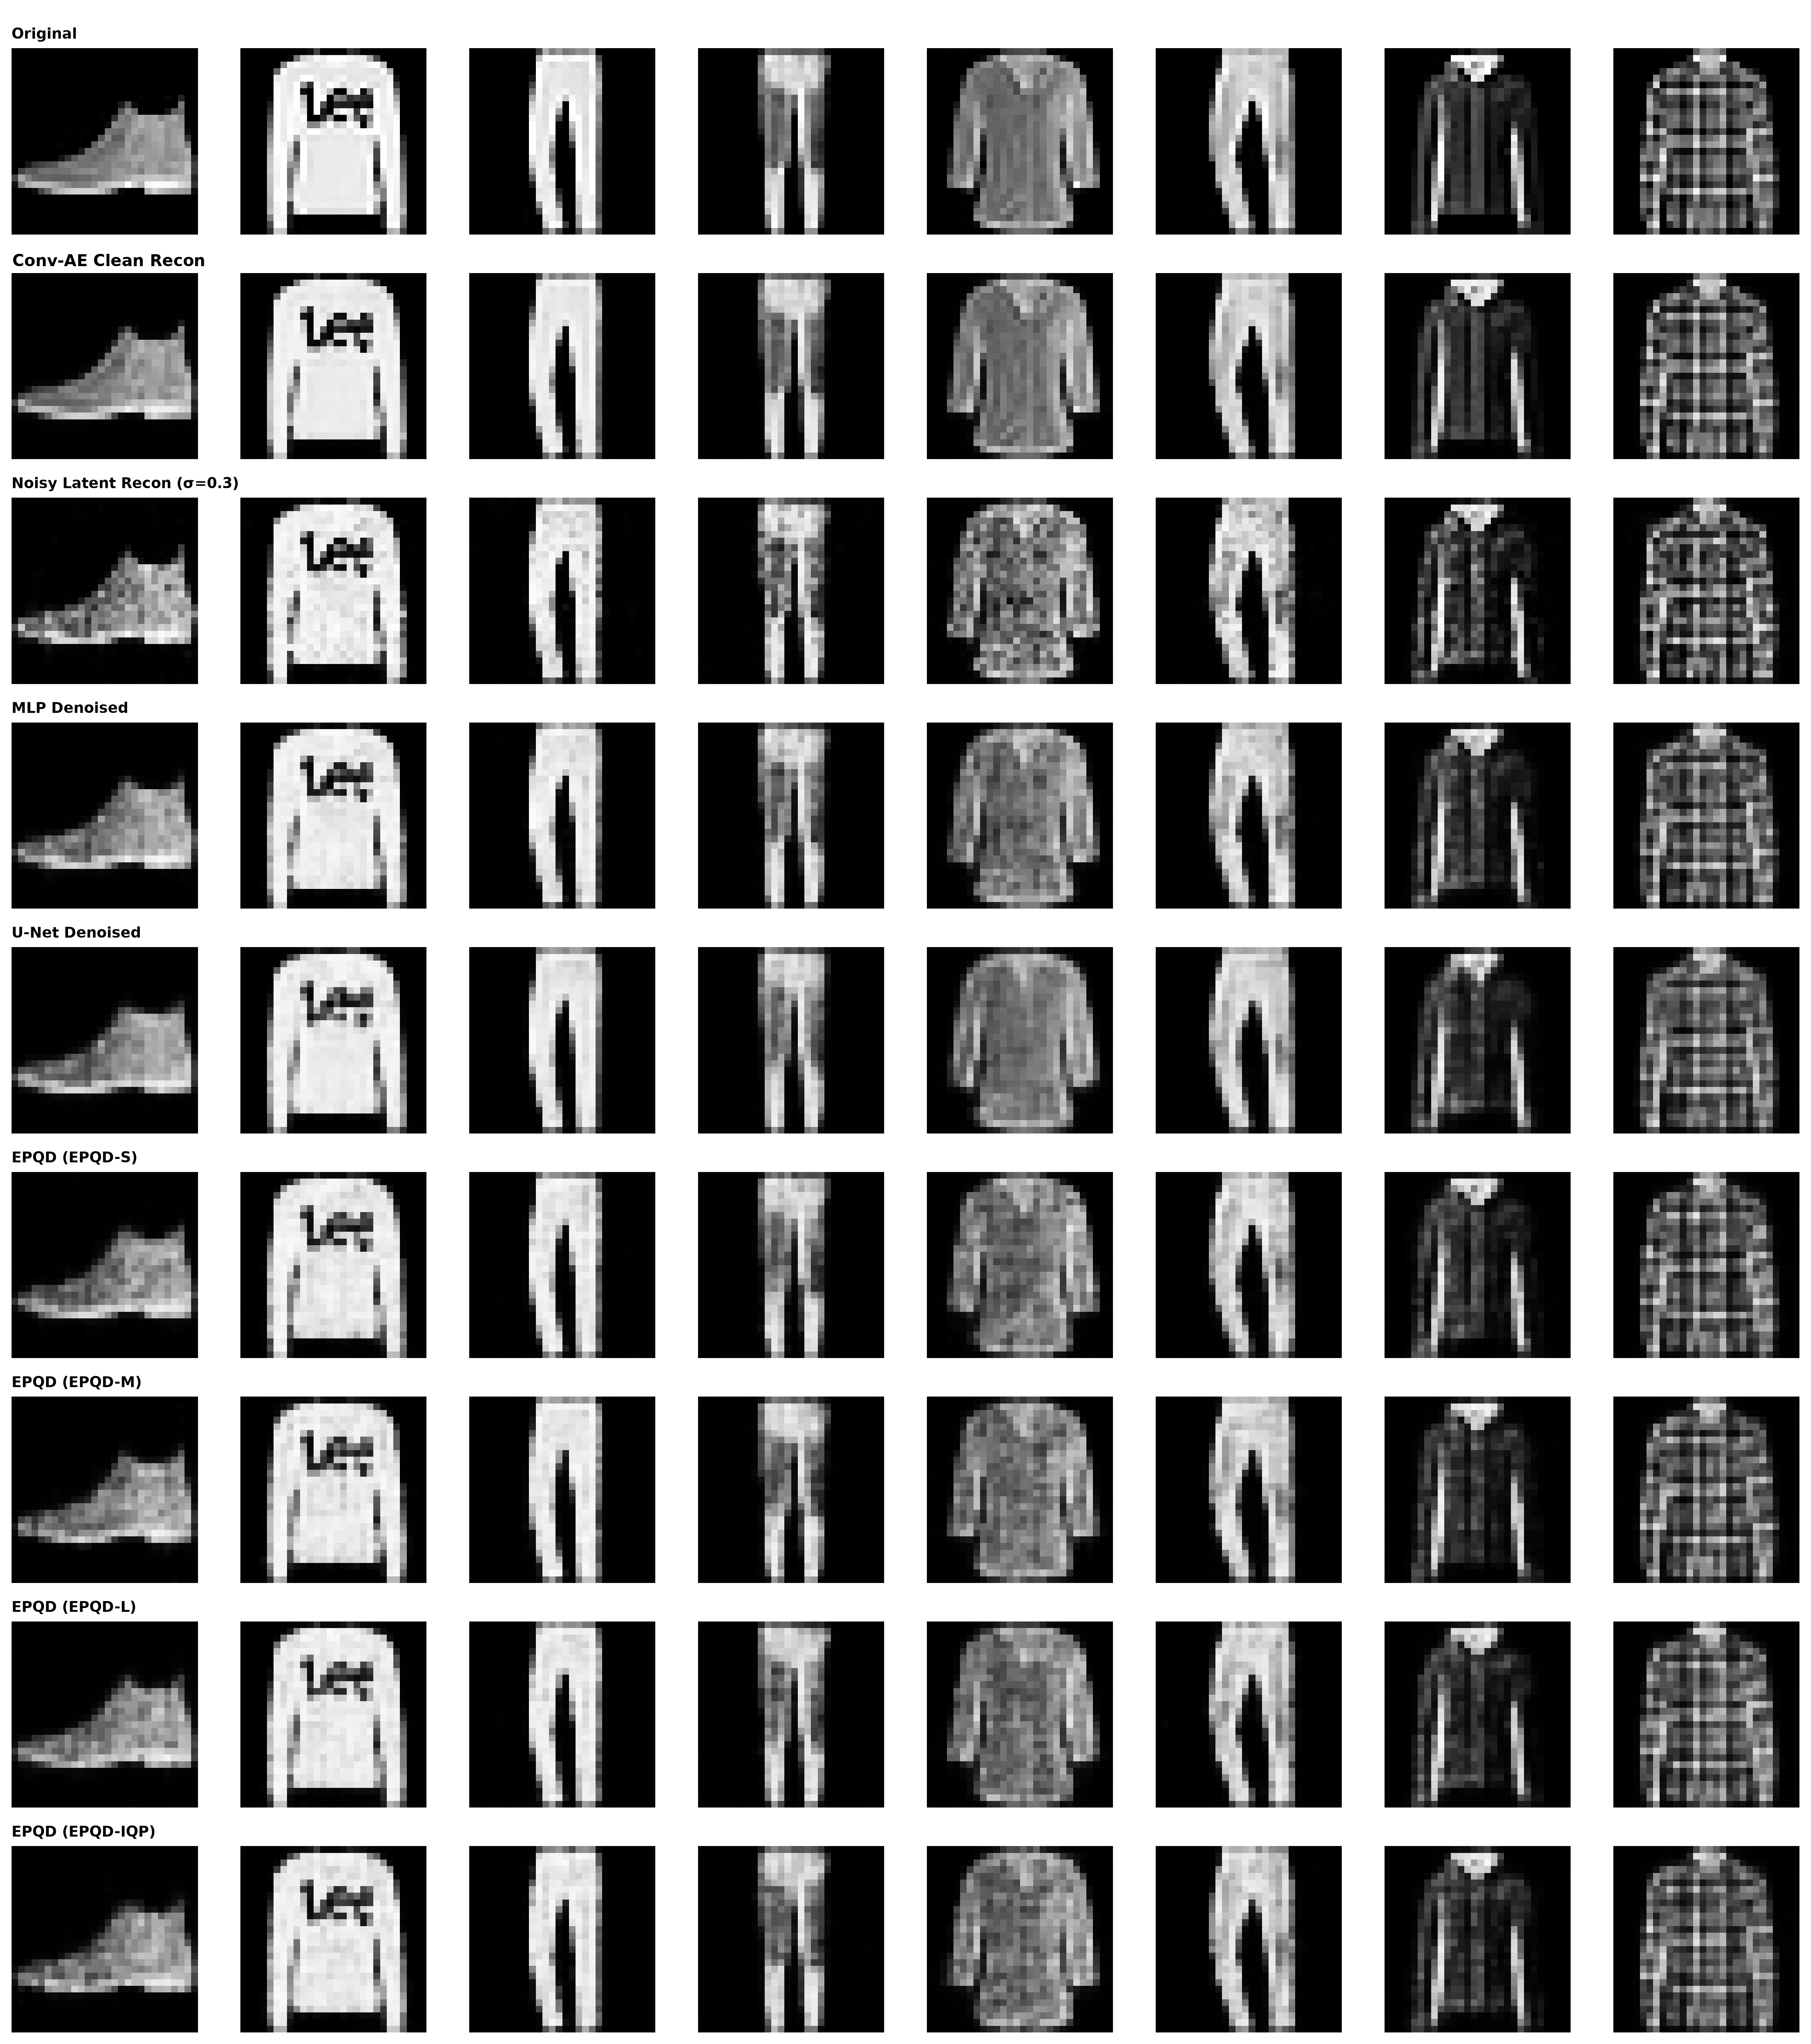
\includegraphics[width=0.72\textwidth]{PHQD_full_comparison.png}
\caption{Reconstructions of the original image, the noisy latent, the classical baselines and the EPQD variants.}
\label{fig:qualitative}
\end{figure*}
\subsection{Discussion}
Deeper circuits help only slightly: going from one to three layers lowers the image MSE from 0.00300 to 0.00294. The IQP-style encoding is not better than the basic ring circuit with the same depth (0.00301 against 0.00298). Each model was trained once, so these small gaps cannot be called significant. The main result is that the best classical baseline, the MLP, beats every 4-qubit hybrid model, which agrees with the finding of Bowles et al.~\cite{bowles} that strong classical models are hard to beat. This is also why classical baselines and ablations are needed before crediting the circuit. EPQD-6Q-V2 changes several things at once (qubit count, repeated encoding, three measurement bases, wider projections, joint stitching fine-tuning and an SSIM loss), so any gain over the 4-qubit models cannot be assigned to the qubit count alone.

\subsection{Computational Cost}
All circuits are simulated on the classical \texttt{default.qubit} simulator with batched evaluation and backpropagation, which avoids one circuit call per patch. No physical quantum hardware was used. The wall-clock times and memory use are [fill in from your logs].

\section{Limitations}\label{sec:limitations}
This study has several limitations. All circuits are run on a classical simulator, so the results do not show how the models would perform on a noisy quantum processor. To keep the simulation fast, the denoisers are trained on part of the data, and the quantum fine-tuning uses at most 8{,}000 patches. The image-level metrics come from small test batches (32 images for the main comparison and 64 for the V2 benchmark), and the FID uses 1{,}000 images. Each model was trained once at a single noise level on one dataset, so the small differences between the 4-qubit models are not statistically established. The classical layers have far more parameters than the circuit, and we did not include a parameter-matched classical replacement, so the gain cannot be credited to the circuit alone. EPQD-6Q-V2 also changes several design choices at once, so its result cannot be attributed to the qubit count. Finally, the autoencoder limits the final image quality, since no denoiser can do better than the decoded clean latent map. Repeating the experiments with several random seeds, noise levels and datasets would give stronger evidence.

\section{Conclusion and Future Work}
This work describes PHQD, a modular patch-based hybrid quantum--classical latent denoising pipeline for Fashion-MNIST. The system uses a convolutional autoencoder to obtain compact latent maps, overlapping patch extraction to create 256-dimensional patch vectors, and EPQD models to estimate clean latent patches. The implementation includes four standard four-qubit circuit configurations and a separate six-qubit V2 system with data re-uploading, Pauli-$X/Y/Z$ readout, and joint refinement with StitchingCNN. Classical MLP and U-Net models provide reference baselines. The final conclusion must state which model performed best on the measured benchmark and quantify the difference using the exact experimental outputs. Future work includes larger evaluation batches, repeated-seed testing, additional datasets and noise levels, hardware-aware simulation, and deployment on quantum devices.
\begin{thebibliography}{17}
\bibitem{ho}
J. Ho, A. Jain, and P. Abbeel,
Denoising diffusion probabilistic models.
In: Advances in Neural Information Processing Systems 33, 6840--6851 (2020).

\bibitem{rombach}
R. Rombach, A. Blattmann, D. Lorenz, P. Esser, and B. Ommer,
High-resolution image synthesis with latent diffusion models.
In: IEEE/CVF Conference on Computer Vision and Pattern Recognition, 10684--10695 (2022).

\bibitem{cerezo}
M. Cerezo et al.,
Variational quantum algorithms.
Nature Reviews Physics 3(9), 625--644 (2021).

\bibitem{benedetti}
M. Benedetti, E. Lloyd, S. Sack, and M. Fiorentini,
Parameterized quantum circuits as machine learning models.
Quantum Science and Technology 4(4), 043001 (2019).

\bibitem{preskill}
J. Preskill,
Quantum computing in the NISQ era and beyond.
Quantum 2, 79 (2018).

\bibitem{havlicek}
V. Havl\'{\i}\v{c}ek et al.,
Supervised learning with quantum-enhanced feature spaces.
Nature 567(7747), 209--212 (2019).

\bibitem{schuld}
M. Schuld, R. Sweke, and J. J. Meyer,
Effect of data encoding on the expressive power of variational quantum-machine-learning models.
Physical Review A 103(3), 032430 (2021).

\bibitem{mcclean}
J. R. McClean, S. Boixo, V. N. Smelyanskiy, R. Babbush, and H. Neven,
Barren plateaus in quantum neural network training landscapes.
Nature Communications 9, 4812 (2018).

\bibitem{kolle}
M. K\"olle et al.,
Quantum denoising diffusion models.
arXiv:2401.07049 (2024).

\bibitem{cacioppo}
A. Cacioppo, L. Colantonio, S. Bordoni, and S. Giagu,
Quantum diffusion models.
arXiv:2311.15444 (2023).

\bibitem{zhang}
B. Zhang, P. Xu, X. Chen, and Q. Zhuang,
Generative quantum machine learning via denoising diffusion probabilistic models.
Physical Review Letters 132(10), 100602 (2024).

\bibitem{huang}
H.-L. Huang et al.,
Experimental quantum generative adversarial networks for image generation.
Physical Review Applied 16(2), 024051 (2021).

\bibitem{bowles}
J. Bowles, S. Ahmed, and M. Schuld,
Better than classical? The subtle art of benchmarking quantum machine learning models.
arXiv:2403.07059 (2024).

\bibitem{fmnist}
H. Xiao, K. Rasul, and R. Vollgraf,
Fashion-MNIST: A novel image dataset for benchmarking machine learning algorithms.
arXiv:1708.07747 (2017).

\bibitem{unet}
O. Ronneberger, P. Fischer, and T. Brox,
U-Net: Convolutional networks for biomedical image segmentation.
In: Medical Image Computing and Computer-Assisted Intervention, LNCS 9351, 234--241 (2015).

\bibitem{parigi}
M. Parigi, S. Martina, and F. Caruso,
Quantum-noise-driven generative diffusion models.
arXiv:2308.12013 (2023).

\bibitem{salinas}
A. P\'erez-Salinas, A. Cervera-Lierta, E. Gil-Fuster, and J. I. Latorre,
Data re-uploading for a universal quantum classifier.
Quantum 4, 226 (2020).
\end{thebibliography}
\end{document}